\section{Implementation Overview}
\label{sec:implementation}

The safety annex is written in Java as a plug-in for the \gls{osate} \gls{aadl} toolset, which is built on Eclipse.  It is not designed as a stand-alone extension of the language, but works with behavioral contracts specified using the \gls{agree} \gls{aadl} annex~\cite{NFM2012:CoGaMiWhLaLu}. 
The architecture of the safety annex is shown in Figure~\ref{fig:plugin-arch}.

\begin{figure}
	\begin{centering}
		%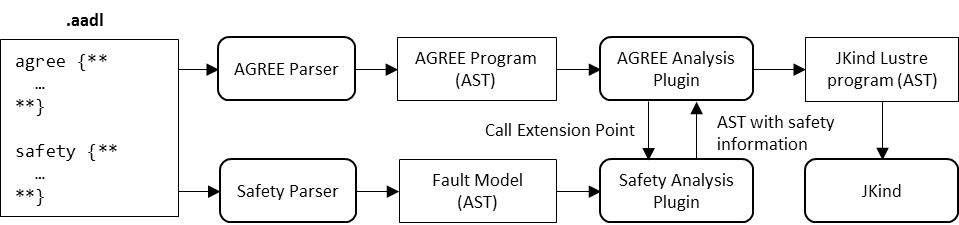
\includegraphics[trim=0 400 430 0,clip,width=0.85\textwidth]{images/arch.png}
		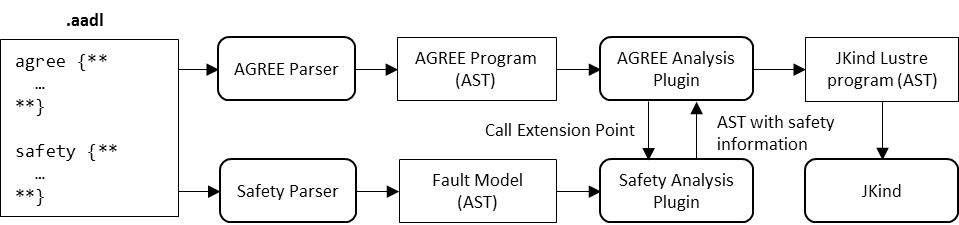
\includegraphics[width=\textwidth]{images/arch.png}
	%\vspace{-0.2in}
	\caption{Safety Annex Plug-in Architecture}
	\label{fig:plugin-arch}
	%\vspace{-0.2in}
	\end{centering}
\end{figure}

\gls{agree} contracts are used to define the nominal behaviors of system components as {\em guarantees} that hold when {\em assumptions} about the values the component's environment are met. When an \gls{aadl} model is annotated with \gls{agree} contracts and the fault model is created using the safety annex, the model is transformed through \gls{agree} into a Lustre model~\cite{Halbwachs91:IEEE} containing the behavioral extensions defined in the \gls{agree} contracts for each system component. 

%This program is intercepted by the Safety Annex plugin and fault model information is added in two ways, depending on which form of fault analysis is being run. 

%\subsection{Verification in the Presence of Faults}
When performing fault analysis, the safety annex extends the \gls{agree} contracts to allow faults to modify the behavior of component inputs and outputs. An example of a portion of an initial \gls{agree} node and its extended contract is shown in Figure~\ref{fig:lustre}. The left column of the figure shows the nominal Lustre pump definition with an \gls{agree} contract on the output. The right column shows the additional local variables for the fault (boxes 1 and 2), the assertion binding the fault value to the nominal value (boxes 3 and 4), and the fault node definition (box 5). Once augmented with fault information, the \gls{agree} model (translated into the Lustre dataflow language~\cite{Halbwachs91:IEEE}) follows the standard translation path to the model checker JKind~\cite{2017arXiv171201222G}, an infinite-state model checker for safety properties. 

\begin{figure}[h!]
	%\hspace*{-2cm}
	%\vspace{-0.3in} 
	\begin{centering}
		%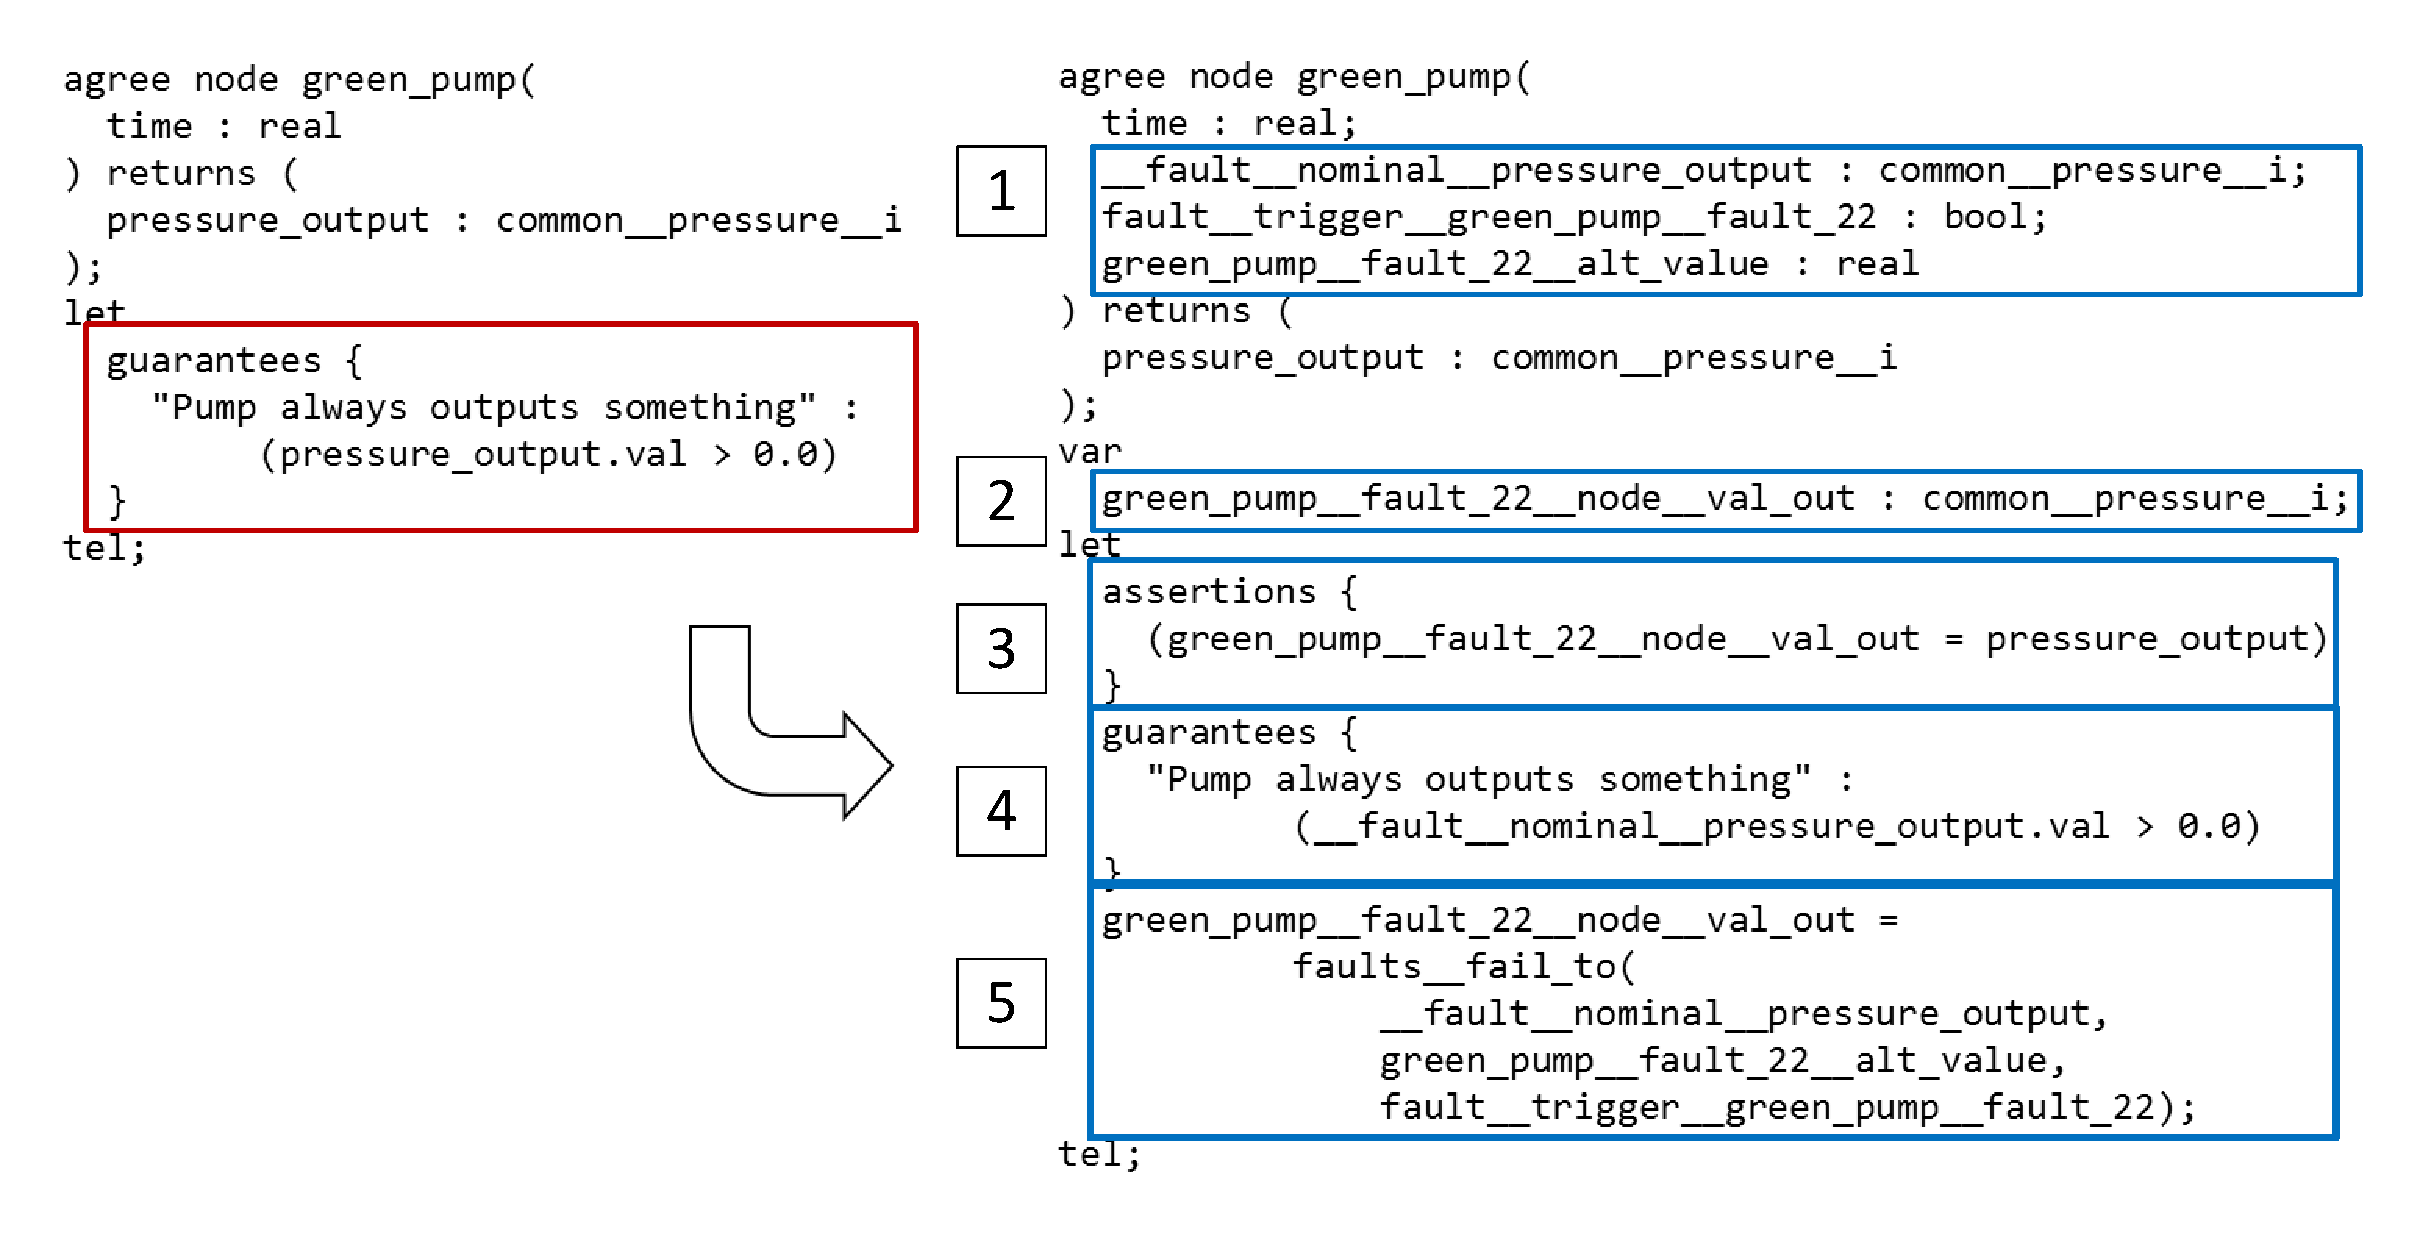
\includegraphics[trim=0 690 -10 70,clip,width=1.5\dimexpr\textwidth-2cm\relax]{images/lustre.pdf}
		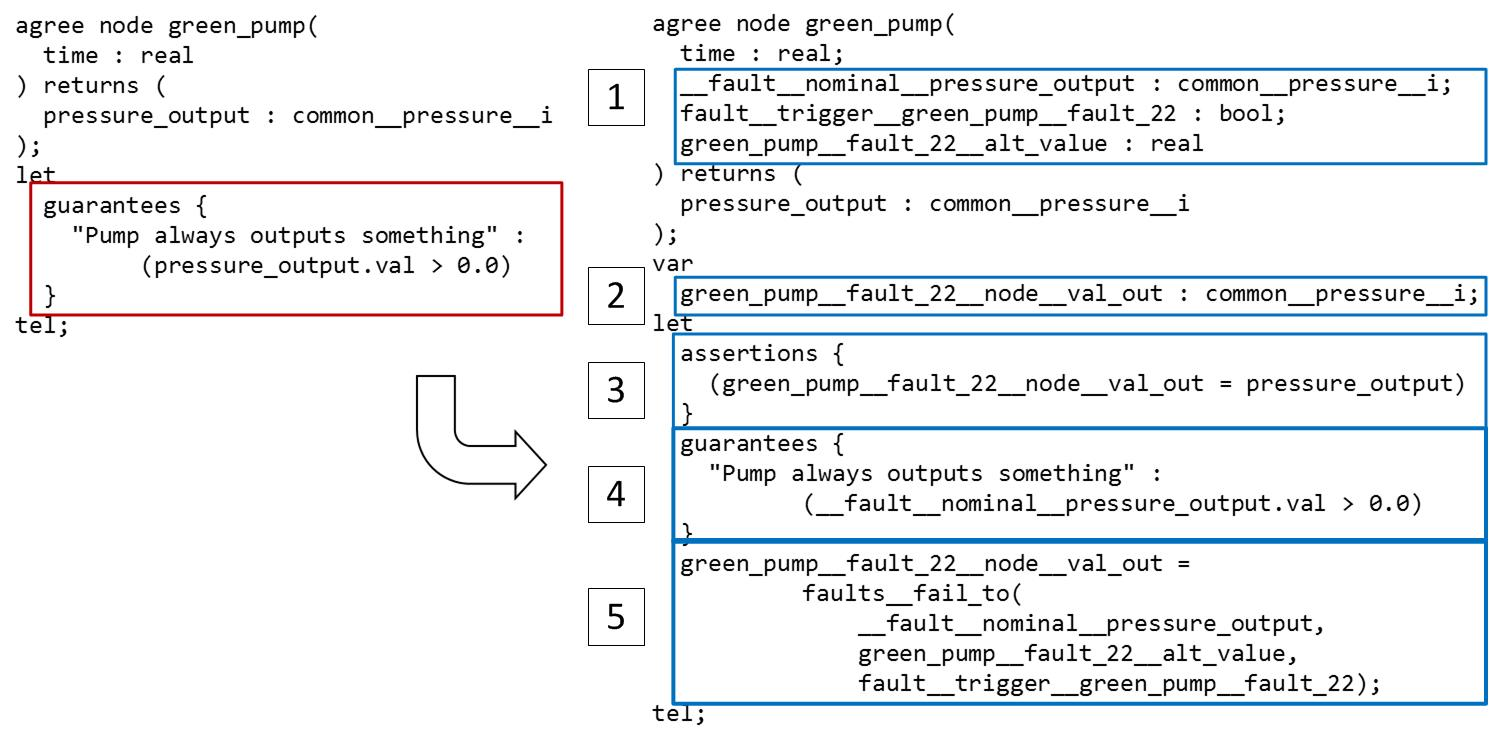
\includegraphics[width=\textwidth]{images/lustre.jpg}
		%\caption{Nominal AGREE node and its extension with faults}
		\caption{Nominal AGREE Node and Extension with Faults}
		\label{fig:lustre}
	%\vspace{-0.3in}
	\end{centering}
\end{figure}

The Lustre formulae are represented in JKind as a transition system, and reasoning is performed using $k$-induction. When performing safety analysis over the model, each fault is defined as an {\em activation literal} and given limited constraint. If the assignment to an activation literal is {\em true}, this corresponds to an active fault and potentially violated guarantee. If that assignment violates a guarantee, then this violation will be reflected in the analysis results. At a system level, it can be seen if a violated guarantee will in turn violate the top level property. Hence it is seen how active faults at leaf level components violate the system level properties. 
 
This analysis approach allows for implicit propagation of violations throughout the system. It also allows for arbitrary temporal activations of faults. There are no explicit constraints put on faults stating when an activation can occur, which allows the model checking procedure free reign to activate the faults at the worst possible times. If there are dependencies regarding fault activations, these are handled through the use of explicit error propagations (see Section~\ref{sec:fault_modeling}). While the model checker may choose various permutations of fault activation, these permutations of faults in terms of exposure time and order of occurrence are not part of the minimal cut set output of this analysis. 

The main constraint put on the model checker in terms of the activation of faults consist of {\em fault hypothesis statements}. These constrain the model by stating either the number of faults that may be active at once, or the overall probability threshold that is allowed. In the latter case, each fault has an associated probability; assuming independence, the probability of a set of faults occurring should not be less than the threshold defined. 

There are two different types of fault analysis that can be performed on a fault model: verification in the presence of faults or the generation of minimal cut sets. The Safety Annex plugin intercepts the AGREE program and adds fault model information depending on which type of fault analysis is being run.

\textbf{Verification in the Presence of Faults}: This analysis returns a counterexample if any guarantee or system level property is violated by active faults in the system. The counterexample shows a concrete scenario why a property is violated, with assignments to each signal in the model by the model checker, possibly over a multi-step progression. The augmentation from Safety Annex to the \gls{agree} program includes traceability information so that when counterexamples are displayed to users, the active faults for each component are visualized.

\textbf{Generate Minimal Cut Sets}: This analysis collects all minimal sets of fault combinations that can cause violation of a property.
%\subsection{Generate Minimal Cut Sets}
Given a complex model, it is often useful to extract traceability information related to the proof, in other words, which portions of the model were necessary to construct the proof. An algorithm was introduced by Ghassabani, et. al. to provide Inductive Validity Cores (IVCs) as a way to determine which model elements are necessary for the inductive proofs of the safety properties for sequential systems~\cite{GhassabaniGW16}. Given a safety property of the system, a model checker can be invoked in order to construct a proof of the property. The IVC generation algorithm extracts traceability information from the proof process and returns a minimal set of the model elements required in order to prove the property. Later research extended this algorithm in order to produce all Minimal Inductive Validity Cores (All-MIVCs) to provide a full enumeration of all minimal set of model elements necessary for the inductive proofs of a safety property~\cite{Ghassabani2017EfficientGO}. 

In this approach, we use the All-MIVCs algorithm to compute the minimal set of model elements (including component contracts and fault activation literals) necessary to prove the top level property, and transform them to minimal sets of faults for the violation of the top level property~\cite{nasaFinalReport}. 

To access the tool plugin, user manual, or models, see the repository located at \small \url{https://github.com/loonwerks/AMASE/}. \normalsize 























